\chapter{Критерии согласия}\label{cha:compl}

\section{Проверка произвольного распределения}\label{cha:compl/sec:nenorm}

\subsection{Тест Колмогорова-Смирнова}\label{cha:compl/sec:nenorm/subsec:kolmsmirn}

\subsubsection*{Теория}\label{cha:compl/sec:nenorm/subsec:kolmsmirn/subsubsection:theory}

Предполагается выборка $X = (X_1, \dots, X_n)$ с непрерывной функцией распределения $F$. Тест применяется при $n \ge 20$.\\
$H_0: F = F_0$ - простая гипотеза. $H_1: F \not = F_0$.\\
$$\begin{gathered}
	T(x) = \sqrt{n} \; \underset{x}{\sup} |\hat{F_n}(x) - F_0 (x)| \xrightarrow[n\to \infty, H_0]{d} \xi \\
	\text{где } \xi \text{ имеет распределение Колмогорова:} \\
	\text{ф.р. } K(t) = \begin{cases}
		\underset{j=-\infty}{\overset{+\infty}{\sum}}(-1)^j e^{-2 j^2 t^2}, \; t >0 \\
		0, t \le 0
	\end{cases}\\
	P(\sqrt{n}\; \underset{x}{\sup} |\hat{F_n}(x) - F_0 (x)| \le t) \xrightarrow[n\to \infty]{H_0} K(t) \\
	C_{\text{кр}} = [K_{1-\alpha}, +\infty]
\end{gathered}$$

\subsubsection*{Пример}\label{cha:compl/sec:nenorm/subsec:kolmsmirn/subsubsection:prob}

\textbf{Проверка на $N(0,1)$}

\begin{lstlisting}[language=Python]
	import numpy as np
	import pandas as pd
	import scipy.stats as stats
	norm_sample = stats.norm.rvs(size=10000)
	stats.kstest(norm_sample, stats.norm.cdf)
	stats.kstest(norm_sample, 'norm')
\end{lstlisting}

\textbf{Проверка на $N(1,4)$}

\begin{lstlisting}[language=Python]
	import numpy as np
	import pandas as pd
	import scipy.stats as stats
	def N_1_4_cdf(x):
    	return stats.norm.cdf(x, loc=1, scale=2)
	
	stats.kstest(norm_sample, N_1_4_cdf)
	stats.kstest(norm_sample, lambda x: stats.norm.cdf(x, loc=1, scale=2))
\end{lstlisting}

\subsection{Тест Андерсона-Дарлинга}\label{cha:compl/sec:nenorm/subsec:andersondarling}

\subsubsection*{Теория}\label{cha:compl/sec:nenorm/subsec:andersondarling/subsubsection:theory}

($\Omega^2$-критерий)\\

Тест работает для $N(0,1)$, $Exp(1)$ и еще пары распределений. Тест выдает значение статистики, набор квантилей вида $x_{1-\alpha}$ и набор соответствующих значений $\alpha$ (в $\%$).\\

$X = (X_1, \dots, X_n)$ - непрерывная функция распределения $F$. $H_0: F = F_0$ - простая гипотеза.
$$\begin{gathered}
	\Omega^2 = \underset{-\infty}{\overset{+\infty}{\int}}\frac{\left( \hat{F_n}(x) - F_0 (x) \right)^2}{F_0 (x) (1 - F_0 (x))} d F_0 (x) \\
	T (x) = n \cdot \Omega^2 \xrightarrow[H_0]{d} \xi, \; P(n \Omega^2 \le x) \xrightarrow[H_0]{}A(x), \; A(Z_p) = p
\end{gathered}$$

\subsubsection*{Пример}\label{cha:compl/sec:nenorm/subsec:andersondarling/subsubsection:prob}

\textbf{Проверка на $N(0,1)$}

\begin{lstlisting}[language=Python]
	import numpy as np
	import pandas as pd
	import scipy.stats as stats
	norm_sample = stats.norm.rvs(size=10000)
	stats.anderson(norm_sample, 'norm')
\end{lstlisting}

\textbf{Проверка на $Exp(1)$}

\begin{lstlisting}[language=Python]
	import numpy as np
	import pandas as pd
	import scipy.stats as stats
	norm_sample = stats.norm.rvs(size=10000)
	stats.anderson(exp_sample, 'expon')
\end{lstlisting}

\subsection{Критерий Пирсона (хи-квадрат)}\label{cha:compl/sec:nenorm/subsec:pirson}

\subsubsection*{Теория}\label{cha:compl/sec:nenorm/subsec:pirson/subsubsection:theory}

Полиномиальная схема: $n$ независимых испытаний, $r$ исходов $A_1, \dots, A_r$. $H_0:$ вероятности исходов $p_1^0, \dots, p_r^0$. Пусть исходы встретилиись $m_1, \dots, m_r$ раз. Статисика:
$$\begin{gathered}
	\hat{\chi^2} = T(x) = \underset{i=1}{\overset{r}{\sum}}\frac{(m_i - n p_i^0)^2}{n p_i^0} \xrightarrow[H_0]{d}\chi^2 (r-1) \\
	C_{\text{кр}} = [\chi_{1-\alpha}^2 (r-1), +\infty)
\end{gathered}$$
Тест применяется при $n \ge 50$ и $m_i \ge 5$.\\

\textbf{Критерий $\chi^2$-Фишера}:
$$\begin{gathered}
	p_i^0 (\theta_1, \dots, \theta_k), \; \theta = (\theta_1, \dots, \theta_k) \in \Theta \\
	\hat{\theta} = arg \; \underset{\theta \in \Theta}{max} \; \underset{j=1}{\overset{r}{\Pi}} \left( p_j^0 (\theta) \right)^{m_j} \text{ -- ОМП} \\
	\hat{\chi^2} = \underset{i=1}{\overset{r}{\sum}}\frac{\left( m_i - n p_i^0 (\hat{\theta}) \right)^2}{n p_i^0 (\hat{\theta})} \xrightarrow[H_0]{d}\chi^2 (r-1-k), \text{ где } k \text{ - кол-во неизвестных параметров}
\end{gathered}$$

В качестве $A_1, \dots, A_r$ берем попадание $X_1, \dots, X_n$ в некоторые множества $\triangle_1, \dots, \triangle_r$. В каждом интервале $\ge 5$ попаданий.

\begin{example}[(критерий Пирсона)]\label{lec:comp/example:1}
	$X = (X_1, \dots, X_n), \; H_0: F = F_0$ - простая гипотеза.
	\begin{center}
		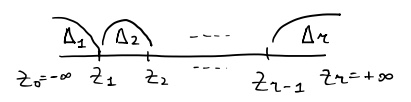
\includegraphics[scale=0.7]{comp1}
	\end{center}

	$m_i$: число $X_i$ в $\triangle_i$.\\
	$p_i^0 = P_0 (X_i \in \triangle_i) = F_0 (Z_i) - F_0 (Z_{i-1})$ (если верна $H_0$)\\
	$$\hat{\chi^2} = \underset{i=1}{\overset{r}{\sum}}\frac{(m_i - n p_i^0)^2}{n p_i^0} \xrightarrow[H_0]{d}\chi^2 (r-1)$$
\end{example}
\begin{example}[(критерий Фишера)]\label{lec:comp/example:2}
	$X = (X_1, \dots, X_n), \; H_0: F = F_0 (\theta_1, \dots, \theta_k)$.
	$$\hat{\chi^2} = \underset{i=1}{\overset{r}{\sum}}\frac{\left( m_i - n p_i^0 (\hat{\theta_1}, \dots, \hat{\theta_k}) \right)^2}{n p_i^0 (\hat{\theta_1}, \dots, \hat{\theta_k})} \xrightarrow[H_0]{d} \chi^2 (r-1-k)$$
\end{example}

\subsubsection*{Пример}\label{cha:compl/sec:nenorm/subsec:pirson/subsubsection:prob}

\textbf{Проверка на $N(0,1)$}

\begin{lstlisting}[language=Python]
	import numpy as np
	import pandas as pd
	import scipy.stats as stats
	
	def chisquare_normality_test(d, loc=None, scale=None, 
			min_bin_value=-3, max_bin_value=3, nbins=17):
	    :param d: array like -- initial data
	    :param loc: loc parameter of norm distribution
	    if loc is None then d.mean() is used
	    :param scale: scale parameter of norm distribution
	    if scale is None then d.std(ddof=0) is used
	    :param min_bin_value: right bound of the first bin
	    :param max_bin_value: left bound of the last bin
	    :param nbins: number of bins
    
	    bins = [-np.inf] + list(np.linspace(min_bin_value, max_bin_value, 
	    		max(nbins-1, 2))) + [np.inf]
	    
	    if loc is None and scale is None:
	        degrees_of_freedom = 2
	    elif loc is not None and scale is not None:
	        degrees_of_freedom = 0
	    else:
	        degrees_of_freedom = 1
	        
	    sf = np.histogram(d, bins)[0]
	    
	    loc = loc or d.mean()
	    scale = scale or d.std(ddof=0)

	    tf = [stats.norm.cdf(bins[i], loc=loc, scale=scale) - 
	    		
	    		stats.norm.cdf(bins[i-1], loc=loc, scale=scale) 
	                   for i in range(1, len(bins))]
	    tf = np.array(tf)*len(d)
	    
	    return stats.chisquare(sf, tf, ddof=degrees_of_freedom), 
	    		stats.chisquare(sf, tf, ddof=0)

	chisquare_normality_test(t_sample, nbins=27)
	chisquare_normality_test(norm_sample, loc=0, scale=2)
\end{lstlisting}

\section{Проверка на нормальность}\label{cha:compl/sec:norm}

\subsection{Тест Шапиро-Уилка}\label{cha:compl/sec:norm/subsec:shapiro}

\subsubsection*{Теория}\label{cha:compl/sec:norm/subsec:shapiro/subsubsection:theory}

Это наиболее мощный критерий проверки нормальности: $P(H_1|H_1) \to max$ среди всех. Работает корректно при $n < 5000$.
$$\begin{gathered}
	H_0: F \in \{N(a, \sigma^2)\}\\
	W = \frac{\left( \underset{i=1}{\overset{t}{\sum}}a_{n-i+1} (X_{(n-i+1)} - X_{(i)}) \right)^2}{\underset{i=1}{\overset{n}{\sum}}(X_i - \overline{X})^2}\\
	t = \begin{cases}
		\frac{n}{2}, \text{ если } n\% 2 =0 \\
		\frac{n-1}{2}, \text{ если } n\% 2 =1
	\end{cases}
\end{gathered}$$
При $H_0$ $W$ имеет табличное распределение, $C_{\text{кр}} = (-\infty, W_{\alpha})$.

\subsubsection*{Пример}\label{cha:compl/sec:nenorm/subsec:shapiro/subsubsection:prob}

\begin{lstlisting}[language=Python]
	stats.shapiro(norm_sample)
\end{lstlisting}

\subsection{Тест Харке-Бера}\label{cha:compl/sec:norm/subsec:ber}

\subsubsection*{Теория}\label{cha:compl/sec:norm/subsec:ber/subsubsection:theory}

$$\begin{gathered}
	H_0: F(x) \in \{N(a, \sigma^2)\} \\
	JB = \frac{n}{6} \left( (S_k)^2 + \frac{1}{4} (K_n)^2 \right) \\
	S_k = \frac{\hat{\mu_3}}{(\hat{\mu_2})^{\frac{3}{2}}}, \text{ Skewness - коэффициент ассиметрии} \\
	K_n = \frac{\hat{\mu_4}}{(\hat{\mu_2})^2}-3, \text{ Kurtosis - коэффициент эксцесса}\\
	\hat{\mu_j} = \frac{1}{n}\underset{i=1}{\overset{n}{\sum}}(X_i - \overline{X})^j
\end{gathered}$$
$$as = \frac{\mu_3}{(\mu_2)^{\frac{3}{2}}}, \text{ степень симметричности}$$
\begin{center}
	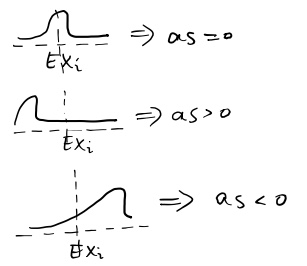
\includegraphics[scale=0.6]{comp2}
\end{center}
$$ex = \frac{\mu_4}{(\mu_2^2)}-3, \text{ степень остроконечности}$$
\begin{center}
	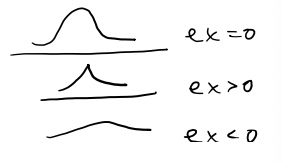
\includegraphics[scale=0.6]{comp3}
\end{center}

Тест работает корректно при $n > 2000$, тогда можно считать, что $JB \Hosim \chi^2 (2)$. Если $n < 2000$, то нужно смотреть таблицу квантилей.

\subsubsection*{Пример}\label{cha:compl/sec:nenorm/subsec:ber/subsubsection:prob}

\begin{lstlisting}[language=Python]
	stats.jarque_bera(norm_sample)
	res = stats.jarque_bera(norm_sample)
	statistics = res[0]
	p_value = 1 - stats.chi2.cdf(statistics, 2)
	p_value
\end{lstlisting}

\subsection{Тест Лиллиефорса}\label{cha:compl/sec:norm/subsec:lilli}

\subsubsection*{Теория}\label{cha:compl/sec:norm/subsec:lilli/subsubsection:theory}

До сих пор находится в разработке, периодически выдает ошибки (чаще всего на выборках объема больше 900). Если p-value получается больше 0.2, то выдает 0.2.\\
$H_0: F(x) = F_0 (x)$ - функция распределения $N(a, \sigma^2)$ - сложная гипотеза, параметры $a$ и $\sigma$ неизвестны. ($H_0: F \in \{N(a, \sigma^2)\}$)
$$\begin{gathered}
	T(x) = \sqrt{n} \; \underset{x}{sup} \; |\hat{F_n}(x) - F(x)| \\
	C_{\text{кр}} = [X_{1-\alpha}, +\infty), \; n > 30
\end{gathered}$$
$F(x)$ - функция распределения $N(\overline{X}, \hat{\sigma^2})$, $\overline{X}$ - ОМП, а для $\hat{\sigma^2}$ - $\frac{1}{n}\underset{i=1}{\overset{n}{\sum}}(X_i - X)^2$.\\
$F(x) = \Phi (\frac{X - \overline{X}}{\hat{\sigma}})$ - распределение Лиллиефорса.

\subsubsection*{Пример}\label{cha:compl/sec:nenorm/subsec:lilli/subsubsection:prob}

\begin{lstlisting}[language=Python]
	from statsmodels.stats.diagnostic import lilliefors
	short_t_sample = stats.t.rvs(4, size=800)
	lilliefors(short_t_sample)
\end{lstlisting}

\subsection{QQ Plot}\label{cha:compl/sec:norm/subsec:qq}

\subsubsection*{Теория}\label{cha:compl/sec:norm/subsec:qq/subsubsection:theory}

(Quantile Quantile Plot - вероятностная бумага)\\

\textbf{Проверка на $N(0,1)$}\\

$X = (X_1, \dots, X_n)$ из $N(0,1)$? $\Phi (x)$ - функция распределения $N(0,1)$. $\hat{F_n}(x) \approx \Phi(x)$. $\Phi^{-1} (\hat{F_n} (X_i)) \approx \Phi^{-1} (\Phi (X_i)) = X_i$. Рассмотрим точки $\left( \Phi^{-1} (\hat{F_n} (X_i)), \; \hat{F_n}^{-1}(\hat{F_n}(X_i)) \right)$, где первая координата - теоретический квантиль, а вторая - выборочный квантиль.
\begin{center}
	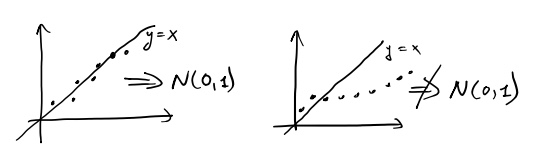
\includegraphics[scale=0.6]{comp4}
\end{center}

\textbf{Проверка на $N(a,\sigma^2)$}\\

$X = (X_1, \dots, X_n)$ из $N(a,\sigma^2)$? Вместо $y=x$ хотим увидеть $y = \sigma x + a$. $\hat{F_n}(x) \approx F_{N(a, \sigma^2)}(x)$. $\Phi^{-1} (\hat{F_N} (X)) \approx \Phi^{-1} (F_N (X)) = \Phi^{-1} (\Phi (\frac{X-a}{\sigma})) = \frac{X - a}{\sigma}$. Рассмотрим точки $\left( \frac{X_i - a}{\sigma}, X_i \right)$.
\begin{center}
	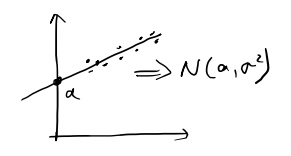
\includegraphics[scale=0.7]{comp5}
\end{center}

\subsubsection*{Пример}\label{cha:compl/sec:nenorm/subsec:qq/subsubsection:prob}

\begin{lstlisting}[language=Python]
	stats.probplot(norm_sample, plot=plt);
\end{lstlisting}

\subsection{Bootstrap}\label{cha:compl/sec:norm/subsec:bootstrap}

\subsubsection*{Теория}\label{cha:compl/sec:norm/subsec:bootstrap/subsubsection:theory}

Асимптотический ДИ:
$$\sqrt{n} \; (\hat{\theta_n} - \theta) \xrightarrow[]{d} N(0, \sigma^2(\theta)) \text{ -- АНО } \hat{\theta_n}$$
Проблемы:
\begin{itemize}
	\item[1)] $\sigma^2(\theta)$ сложно посчитать
	\item[2)] не знаем распределения выборки $X_i$
	\item[3)] $n$ не бесконечно большое
\end{itemize}
$X = (X_1, \dots, X_n)$ - выборка с неизветсной функцией распределения $F$.
$$T_n (X_1, \dots, X_n) \; \leftarrow \; \hat{\theta_n} (X_1, \dots, X_n) \text{ АНО}$$
Например, хотим оценить $D T_n$.\\

\textbf{Этап 1}\\
Рассмотрим реализацию $X_1, \dots, X_n$:
\begin{tabular}{| l | c | r |}
	\hline
	$X_1$ & $\dots$ & $X_n$ \\ \hline
	$\frac{1}{n}$ & $\dots$ & $\frac{1}{n}$ \\ \hline
\end{tabular} - дискретное распределение, это функция распределения $\hat{F_n}(x)$ (ЭФР).\\
Bootstrap -- создание одной или нескольких выборок $\hat{F_n}$ объема $n$. $\hat{F_n}(x) \approx F(x)$.\\

\textbf{Этап 2}\\
$D T_n$ -- ?\\
Сэмплируем $m$ бутстрэпных выборок: $\{ X_{i,1}^{*} \}_{i=1}^n, \dots,  \{X_{i,m}^{*} \}_{i=1}^n $. Вычисляем статистику на выборках: $T_{n,1}^{*}, \dots, T_{n,m}^{*}$. 
$$V_{boot} (T) = \hat{D T_n} = \frac{1}{m} \underset{j=1}{\overset{m}{\sum}}\left( T_{n,j}^{*} - \frac{1}{m}\underset{l=1}{\overset{m}{\sum}}T_{n,l}^{*} \right)^2, \;\; T^{*} = \frac{1}{m}\underset{l=1}{\overset{m}{\sum}}T_{n,l}^{*}$$

\textbf{Этап 3}\\
$T_n$ для АДИ:
$$\left( T_n - Z_{\frac{1+\gamma}{2}} \cdot \sqrt{V_{boot}(T)}, \; T_n + Z_{\frac{1+\gamma}{2}} \cdot \sqrt{V_{boot}(T)} \right)$$

\subsubsection*{Пример}\label{cha:compl/sec:nenorm/subsec:bootstrap/subsubsection:prob}

\begin{lstlisting}[language=Python]
	sample = pd.read_csv("Bootstrap_sample.txt")
	sample = sample['sample']
	n = len(sample)

	bootstrap = np.random.choice(sample, size=(100, n))
	v_boot = np.percentile(bootstrap, 50, axis=1).var()
	np.percentile(bootstrap, 50, axis=1)
	gamma=0.9
	g = (1 + gamma)/2.0
	(
    np.percentile(sample, 50) - stats.norm.ppf(g) * np.sqrt(v_boot),
    np.percentile(sample, 50) + stats.norm.ppf(g) * np.sqrt(v_boot)
	)
\end{lstlisting}















